\documentclass[10pt,twocolumn,letterpaper]{article}
\usepackage[T1]{fontenc}
\usepackage[review]{cvpr}
\usepackage{graphicx,amsmath,amssymb,booktabs,microtype,longtable}
\usepackage[breaklinks,colorlinks,allcolors=black]{hyperref}
\def\confName{CVPR}\def\confYear{2027}
\title{Seeing Motion Is Not Identifying Mechanics:\\Supplementary Evidence and Preserved Platform Studies}
\author{Anonymous manuscript}
\newcommand{\R}{\mathbb{R}}
\begin{document}
\maketitle
\section{Reading this supplement}
The first part documents the new joint-field identification campaign. It distinguishes the exact finite model, approximate continuous inference, and a separately frozen hierarchical-force-scale study. The final part reproduces the previous platform supplement unchanged, preserving nonlinear contacts, rendering studies, public-data comparisons and their negative results. The archived experiments use different adapters; their results are not outputs of the newly marginalized joint-field posterior.

The new reference is a known-geometry, known-camera, known-correspondence, small-strain quasistatic experiment. Observations are noisy projected displacements. Its rendered surfaces visualize mechanical states; they do not constitute RGB reconstruction quality measurements. Loading times index correlated quasistatic experiments, not an integrated dynamic trajectory. Original unobserved times are interpolation because initial observations include times 0,3,7. New-load targets are independent reset experiments under known loads, not future frames with unknown actions.

\section{Coordinates, units and discretization}
Both objects have bounding box $[-.06,.06]\times[-.03,.03]\times[0,.06]$ metres. The stepped object removes the upper-right quarter of the longitudinal/vertical bounding rectangle ($x>0$, $z>.03$ m), leaving 75\% of the bounding volume. A regular grid is split into six tetrahedra per cell, consistently oriented. The primary grid uses $(8,4,4)$ cells:225 nodes/768 tetrahedra for block and 185 nodes/576 tetrahedra for step. Fine truth uses $(12,6,6)$ cells. Density is 500 kg/m$^3$, but is not identified and does not enter quasistatic equilibrium. Poisson ratio is 0.30. Gravity is omitted in the incremental reference; the symmetry argument must not be transferred unchanged to a known, nonzero gravitational load.

For linear tetrahedra, element stiffness is assembled from the exact constant shape gradients and isotropic Lam\'e coefficients. Elastic stiffness has the expected rigid modes. The only anchoring is the declared positive distributed Gaussian support. There is no hidden diagonal jitter or fixed corner. Cholesky factorization failures would be failures of the declared solve, not silently repaired changes to the model.

Surface integrals use three degree-two quadrature points per triangular face. Gaussian traction weights are normalized over the relevant surface and scattered through the face shape functions; each mode sums to a unit force. Support stiffness uses a lumped nodal diagonal from the same normalized quadrature. This is a declared discretization, not the consistent surface mass matrix. Normalization preserves total force under refinement but does not guarantee a converged displacement field.

\section{Material and interaction families}
Material kernel centers are $(-.035,0,.03)$ and $(.035,0,.03)$ metres, with scales $(.035,.06,.06)$ metres. Normalized kernel values define a partition of unity. Their difference is centered by the element-volume average before multiplying log contrast. Thus the reference modulus parameter is a volume-geometric mean, rather than the arithmetic average of local moduli.

All support/load footprints have a fixed longitudinal width 0.018 m and are broad in the other surface coordinate. Unknown support location lies in$[-.025,.025]$m; unknown top/side load location lies in$[-.04,.04]$m and is shared between the two modes. The top footprint on the step includes both horizontal terraces. Support stiffness lies in$[4000,16000]$N/m, reference modulus in$[8000,32000]$Pa, and log contrast in$[-.8,.8]$. Material and support scales have uniform priors in their log coordinates. Five equally spaced values in every coordinate define the primary 3125-component dictionary.

The two unknown traction modes act along$-z$ on the top and$-y$ on a side. Their amplitudes may be positive or negative. Accordingly, these experiments represent applied signed tractions and bilateral compliant supports. They do not discover contact labels, nonpenetration, friction or detachment. A negative top amplitude would require a pulling actuator; it is not an ordinary unilateral poke.

\begin{figure*}[!t]
\centering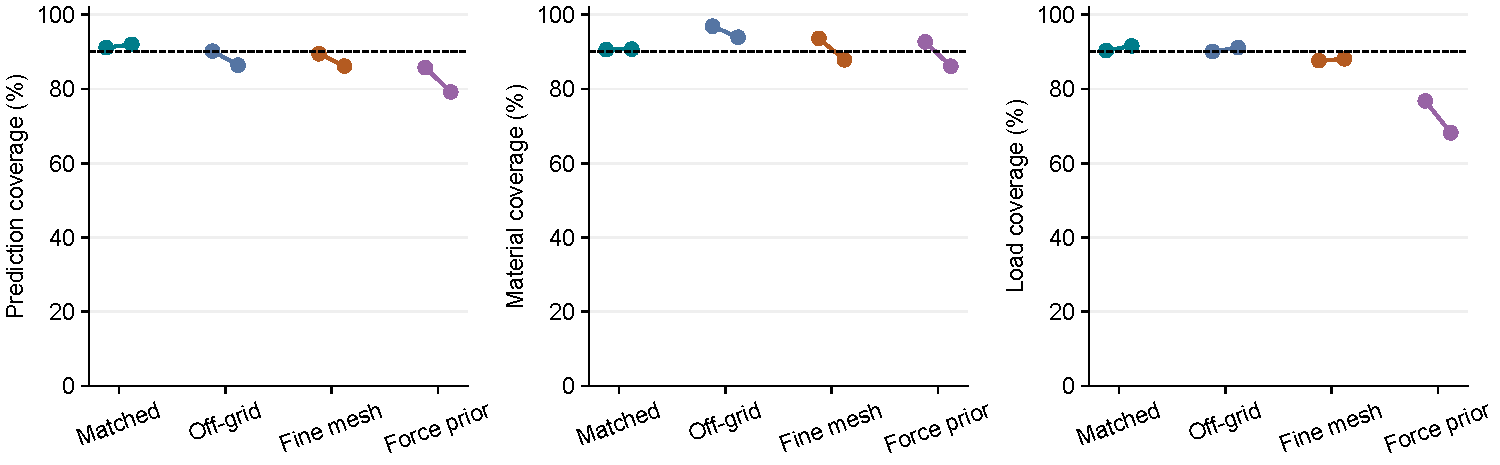
\includegraphics[width=.98\textwidth]{figures/coverage.pdf}
\caption{\textbf{Complete surface-study marginal coverage.} Initial versus four-adaptive-measurement results, including material and load coverage. Same-model calibration and mismatch robustness are distinct tests.}
\end{figure*}

\section{Observations and targets}
Twenty reference points are declared without using any data. Sixteen span$x\in\{-.045,-.015,.015,.045\}$, $y\in\{-.03,.03\}$ and$z\in\{.015,.025\}$m. Four additional points use$x\in\{-.045,-.015\}$, both$y$ values and$z=.05$m. These coordinates lie on the front/back surfaces of both geometries. The primary acquisition and force-scale studies use this surface protocol (v04/v05), as does the temporal follow-up (v06). Earlier v01/v02/v03 reference studies used interior material coordinates at $y=\pm.025$ m and are retained only as mathematical sensor/numerical references. Their order is fixed by the Cartesian-product construction.

Initial measurements use points 1,5,9,13, components$x,z$, and loading times 0,3,7:24 scalar observations. Independent measurement noise has standard deviation$2\times 10^{-5}$m. Two force modes at eight uniformly spaced loading times have a separable Mat\'ern-$3/2$ temporal covariance with correlation length 0.30 and amplitude 0.08 N; directions are a priori independent.

The ten camera candidates are six oblique measurements at back-surface points 3,11 and times 1,4,6, plus four $z$-component measurements at front points 1,13 and times 2,5. For the back view, the outward camera direction is $(-1,1,0)/\sqrt2$ and measured direction is $(1,1,0)/\sqrt2$. Initial/front views use camera direction $(0,-1,0)$. Six calibrated probes use top/side 0.08 N loads at $x=-.04,0,.04$m and measure point 13. Top probes measure $z$ from the front; side probes measure $(1,1,0)/\sqrt2$ with outward camera direction $(1,-1,0)/\sqrt2$. Thus each measured direction lies in its camera image plane. A deformed-surface visibility audit checks all loading times and all six probe states, using explicit ray--triangle intersection, surface membership and outward normals. It checks 27,776 marker/view instances over all 320 primary and 128 hierarchical cases, with zero failures. This verifies geometric visibility of supplied markers, not correspondence correctness or recoverability from RGB. Each candidate yields one scalar, with the same stated noise. Probe measurements use an unloaded/reset object with unchanged material/support parameters. Original loads are replayable for additional camera observations. The cost model does not equate a physical image with a scalar observation or account for actuator complexity.

The predictive target is fixed before action selection. Eight positive-$y$ points, excluding points 3 and 11, at all eight times give 192 original-motion coordinates. The first sixteen reference points under four reset loads at$x=-.02,+.02$m, top/side, give 192 changed-load coordinates. None of the original target points is acquired, and none of the target reset loads is used as an acquisition probe. This prevents a policy from appearing better merely because its chosen measurement became its evaluation target.

\section{Conditional and total uncertainty}
For hypothesis$h$, write$y=H_ha+d_h+\epsilon$, $a\sim\mathcal N(0,\Lambda)$ and$\epsilon\sim\mathcal N(0,R)$. The normalized marginal likelihood is
\begin{equation}
\log p(y\mid h)=-\tfrac 12\{r_h^TC_h^{-1}r_h+\log|C_h|+n\log(2\pi)\},
\end{equation}
with$r_h=y-d_h$ and$C_h=R+H_h\Lambda H_h^T$. Every changing determinant is retained. The finite posterior weights multiply this likelihood by the declared hypothesis prior.

For$q=T_ha+b_h$, conditional means and variances are combined by total expectation and variance. The between-hypothesis term is part of the reported prediction and force uncertainty. Marginal equal-tail intervals invert the full Gaussian-mixture CDF. Deterministic material fields are a weighted discrete distribution; their intervals can be conservative because of atoms. Prediction coverage uses 24 fixed coordinates, material coverage 20 fixed points, and force coverage 16 amplitudes. None is simultaneous whole-field coverage.

The moment-independence ablation preserves the force mean/covariance and the material marginal, but replaces their dependence with one shared moment-matched Gaussian force distribution. Its mean-prediction calculation is a useful dependence control; the ablation is not the exact product of two full mixture marginals. Joint-MAP selects the maximum of$\log w_h-\tfrac 12\log|S_h|$, whereas marginal-MAP selects$\log w_h$. These are different posterior summaries when the conditional covariance changes.

\section{Acquisition calculation and audits}
For scalar action$s$, the component predictive mean is$\mu_{s,h}=h_{s,h}m_h+d_{s,h}$ and variance$v_{s,h}=h_{s,h}S_hh_{s,h}^T+\sigma^2$. Hypothetical observations update Gaussian conditionals and mixture weights. The expected average target variance is estimated with 128 posterior-predictive draws. The same random numbers are used across candidates; acquisition RNG has a separate namespace from truth/noise generation. The selected observation alone updates the actual posterior.

Fixed mixed, camera-only and probe-only schedules are greedily selected from twelve separate development cases per shape using their average realized target squared error. No final case selects these schedules. Random chooses without replacement. All policies receive the same case-specific potential observation noise, making their comparison paired.

\IfFileExists{sections/acquisition-audit-text.tex}{The independent surface audit replays the first four matched cases per geometry, all four decisions, with 1024 predictive draws per candidate. It retains the original actions. 29 of 32 choices agree. Maximum estimated chosen-action regret is 1.529\% of current risk. Two disagreements have descriptive paired 95\% lower bounds above zero, but selecting the audit minimum introduces bias: these are not selection-corrected optimality tests.

A separate diagnostic halves/doubles the assumed force-prior standard deviation while replaying identical original observations and acquired actions. After acquisition, material means change by 30.0\%/22.5\% relative to nominal; predictive means change by 0.0185/0.0098 mm. Nominal 90\% coverage on these eight cases is 91.67\%, compared with 73.96\%/92.71\% under the changed priors. These small-cohort descriptive fractions quantify sensitivity, not population calibration. The separate hierarchy study evaluates uncertainty in amplitude scale on fresh cases.
}{The surface acquisition audit is running.}

\section{Hierarchical force-scale protocol}
A separate fresh cohort samples the same finite spatial prior and one of five equally probable amplitude scales $\tau\in\{.5,1/\sqrt2,1,\sqrt2,2\}$. There are 64 cases per geometry. Conditional forces retain the same temporal correlation. The resulting 15,625-component posterior is evaluated exactly; factorization reuse avoids repeating mechanics solves for different scales. Full mixture distributions, rather than a moment-matched collapse, supply intervals and evidence updates.

Four models receive identical evidence: the hierarchy, fixed nominal scale, a single Gaussian whose variance matches the mixture prior, and an oracle given the true scale. The broader Gaussian's standard-deviation multiplier is $\sqrt{1.55}=1.24499$. Four fixed views (candidate indices 0,2,4,9) and four fixed probes (10,12,13,14) form independent branches from the initial state. Neither branch includes the other branch's observations. No action or hyperprior was selected on this final cohort. Finite-scale posterior endpoint mass should be compared with its prior value 0.4; endpoint mass alone is not evidence of numerical collapse.

\section{Temporal-prior follow-up}
The v04 force-correlation failure motivated a separately frozen v06 follow-up; it does not replace or relabel the original test. There are 32 fresh cases per geometry. True force correlation length is 0.10, and amplitude scale is sampled from the same five-value prior. The expanded estimator mixes lengths $\{0.10,0.30,0.60\}$ and the five scales, giving 46,875 spatial/hyperparameter components. Controls are amplitude-only uncertainty with nominal length 0.30, fixed nominal covariance, and an oracle given true covariance hyperparameters. The oracle does not receive true spatial material/support/load parameters. All methods receive identical original observations and the same separate four-view/four-probe branches.

Fixed true length 0.10 makes this a conditional stress test, not prior-averaged calibration. It is a follow-up to a recognized model error, not an untouched primary evaluation. Exact conditional Gaussian integration and full finite-mixture updates/intervals remain unchanged. An independent dense Gaussian identity audit verifies component indexing, normalized evidence and camera/probe updates to below $5\times10^{-16}$. Error, coverage and interval width are reported together, with every fresh case retained.
\IfFileExists{sections/temporal-results.tex}{\begin{table*}[!t]\centering\small\setlength{\tabcolsep}{4pt}
\caption{Posthoc temporal-prior follow-up, all 64 fresh cases. True correlation length 0.10; conditional stress coverage, not prior-averaged calibration. Force interval width is in N. Fixed views and probes branch independently.}
\begin{tabular}{llrrrrrr}\toprule
Evidence & Model & Hidden mm & Reset mm & Material rel. & Pred. cov. & Force cov. & Width N\\\midrule
initial & scale-correlation & 0.1456 & 0.0311 & 0.518 & 86.6 & 82.1 & 0.202\\
initial & amplitude-only & 0.1550 & 0.0312 & 0.521 & 82.4 & 75.3 & 0.174\\
initial & fixed-nominal & 0.1550 & 0.0322 & 0.506 & 77.2 & 68.4 & 0.135\\
initial & oracle & 0.1379 & 0.0245 & 0.448 & 89.6 & 89.8 & 0.239\\
views & scale-correlation & 0.1007 & 0.0304 & 0.506 & 88.0 & 83.9 & 0.177\\
views & amplitude-only & 0.1170 & 0.0307 & 0.476 & 81.1 & 72.4 & 0.138\\
views & fixed-nominal & 0.1170 & 0.0352 & 0.460 & 70.8 & 59.5 & 0.097\\
views & oracle & 0.0972 & 0.0223 & 0.399 & 91.0 & 91.7 & 0.185\\
probes & scale-correlation & 0.1450 & 0.0130 & 0.306 & 89.5 & 82.6 & 0.183\\
probes & amplitude-only & 0.1541 & 0.0131 & 0.306 & 86.1 & 74.6 & 0.154\\
probes & fixed-nominal & 0.1544 & 0.0157 & 0.331 & 80.3 & 68.8 & 0.127\\
probes & oracle & 0.1373 & 0.0104 & 0.285 & 93.0 & 89.9 & 0.231\\
\bottomrule\end{tabular}
\end{table*}
\begin{figure*}[t]
\centering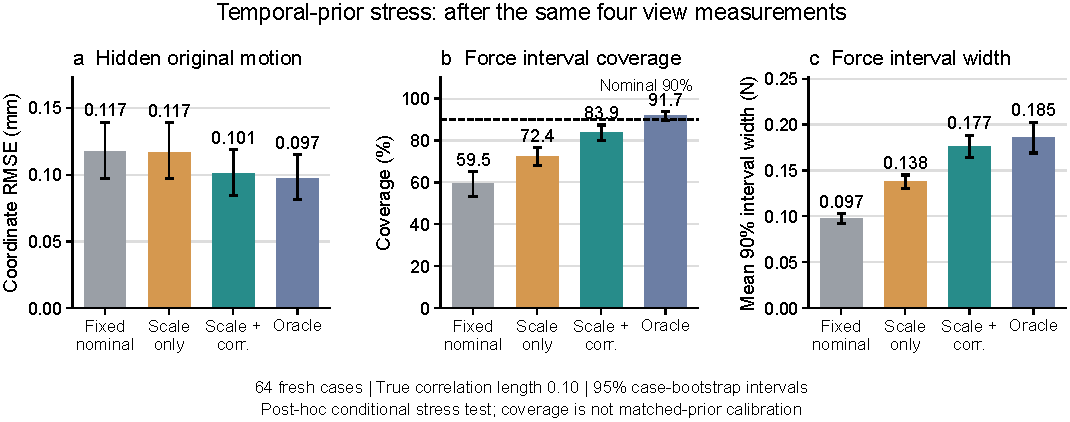
\includegraphics[width=.98\textwidth]{figures/temporal-comparison.pdf}
\caption{\textbf{Temporal uncertainty partially repairs a recognized failure.} Fresh 64-case conditional stress test after four fixed views. Error, coverage and width are shown together, with stratified case-bootstrap 95\% intervals. The covariance oracle is given true amplitude scale and correlation length, not true material or force history.}
\end{figure*}
}{Temporal follow-up evaluation is running.}

\section{Continuous posterior calculation}
Continuous inference uses the same five physical coordinates with a uniform bounded prior in those coordinates. Gaussian load amplitudes remain integrated exactly. Tempering selects the next likelihood exponent using a conditional effective-sample-size criterion. Systematic resampling and reflected random-walk Metropolis moves update particles; bounded proposal adaptation occurs between stages. Rejected or invalid states are not redrawn until valid. Stage-boundary checkpoints include RNG state and target/source fingerprints.

The main continuous cohort uses 32 fresh continuous-prior cases per geometry on the same mesh. Initial, recorded-active-final and recorded-fixed-final evidence are fitted with 1024 particles. The policies were selected by the finite dictionary, not by continuous SMC. A separate diagnostic repeats the first two finite-matched and off-grid-fine cases, both geometries and all three evidence stages, with two independent seeds and 1024/2048 particles. These checks evaluate numerical sensitivity; they do not prove an exact continuous posterior. The finite and continuous priors differ at the boundaries, so posterior disagreement is not solely quadrature error.

\begin{figure*}[!t]
\centering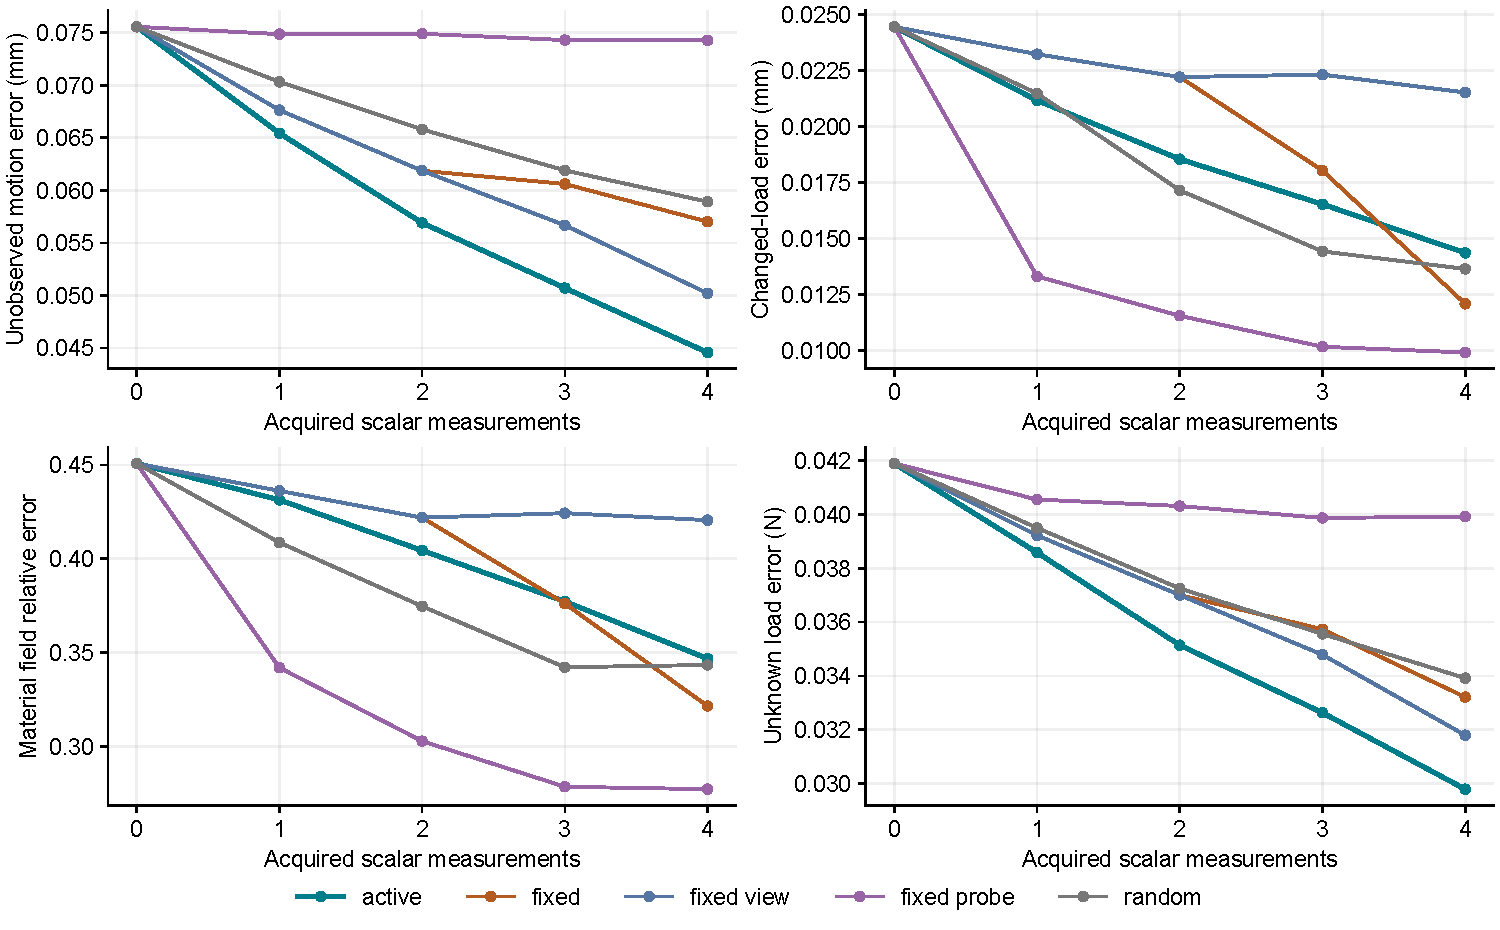
\includegraphics[width=.98\textwidth]{figures/acquisition.pdf}
\caption{\textbf{All primary acquisition endpoints.} Complete matched-cohort trajectories for hidden motion, new loads, material and unknown-force error. Lower combined prediction error does not imply superiority on each component.}
\end{figure*}

\IfFileExists{sections/continuous-posthoc.tex}{\paragraph{Targeted posthoc numerical check.} Sensitivity flags for the block's matched case 1 after fixed measurements motivated two fresh-seed, 4096-particle repeats. The original 1024/2048 runs differ by up to 0.1104 in parameter marginal CDF and 0.0023\,mm in target-mean RMS. Strong support/load and support/stiffness correlations are consistent with inefficient diagonal random-walk exploration; these summaries do not establish a separate missed mode. With the same four Metropolis moves per stage, the two larger runs differ by 0.0403 in CDF and 0.0003\,mm in target-mean RMS, and agree within the original descriptive thresholds. Their final Metropolis acceptance rates are 12.9\%/12.6\%; resampled equal weights are not a convergence diagnostic. The maximum CDF difference between a 4096 run and a lower-count run is still 0.1006. All original flags and fits remain reported. This selected-case follow-up neither replaces the primary cohort nor certifies global convergence.
}{}

\section{Complete new results}
The following tables retain every acquisition policy and representation control, followed by continuous inference, dependence and actual surface-traction diagnostics.
\IfFileExists{sections/supplement-tables.tex}{\begin{table*}[!t]\centering\small\setlength{\tabcolsep}{4pt}
\caption{Matched finite. All errors are means of case-level metrics. Coverage is marginal at nominal 90\%. Point/representation controls use initial evidence; acquisition rows use four additional scalars. Dashes indicate intervals not evaluated for that control.}
\begin{tabular}{lrrrrrrrrr}\toprule
Policy & Cases & Added & Hidden mm & New-load mm & Material rel. & Force N & Pred. cov. & Mat. cov. & Force cov.\\\midrule
Initial & 128 & 0 & 0.0756 & 0.0245 & 0.451 & 0.042 & 91.1 & 90.5 & 90.3\\
active & 128 & 4 & 0.0446 & 0.0144 & 0.347 & 0.030 & 92.0 & 90.7 & 91.6\\
fixed & 128 & 4 & 0.0570 & 0.0121 & 0.322 & 0.033 & 89.2 & 87.7 & 90.8\\
fixed view & 128 & 4 & 0.0502 & 0.0215 & 0.421 & 0.032 & 91.3 & 90.9 & 90.4\\
fixed probe & 128 & 4 & 0.0743 & 0.0099 & 0.277 & 0.040 & 89.1 & 88.0 & 90.6\\
random & 128 & 4 & 0.0589 & 0.0137 & 0.343 & 0.034 & 92.0 & 89.0 & 91.4\\
marginal map & 128 & 0 & 0.0761 & 0.0274 & 0.553 & 0.043 & -- & -- & --\\
joint map & 128 & 0 & 0.0798 & 0.0607 & 0.517 & 0.050 & -- & -- & --\\
uniform material & 128 & 0 & 0.0762 & 0.0258 & 0.471 & 0.042 & -- & -- & --\\
fixed interaction & 128 & 0 & 0.2051 & 0.0495 & 0.666 & 0.134 & -- & -- & --\\
independent moments & 128 & 0 & 0.0759 & 0.0245 & 0.451 & 0.042 & -- & -- & --\\
\bottomrule\end{tabular}
\end{table*}

\begin{table*}[!t]\centering\small\setlength{\tabcolsep}{4pt}
\caption{Continuous coordinates. All errors are means of case-level metrics. Coverage is marginal at nominal 90\%. Point/representation controls use initial evidence; acquisition rows use four additional scalars. Dashes indicate intervals not evaluated for that control.}
\begin{tabular}{lrrrrrrrrr}\toprule
Policy & Cases & Added & Hidden mm & New-load mm & Material rel. & Force N & Pred. cov. & Mat. cov. & Force cov.\\\midrule
Initial & 64 & 0 & 0.0618 & 0.0246 & 0.465 & 0.046 & 90.2 & 96.9 & 90.0\\
active & 64 & 4 & 0.0382 & 0.0172 & 0.393 & 0.033 & 86.4 & 93.9 & 91.1\\
fixed & 64 & 4 & 0.0462 & 0.0163 & 0.397 & 0.037 & 85.9 & 93.3 & 87.9\\
fixed view & 64 & 4 & 0.0422 & 0.0233 & 0.454 & 0.035 & 89.8 & 94.4 & 89.8\\
fixed probe & 64 & 4 & 0.0617 & 0.0149 & 0.386 & 0.045 & 84.5 & 87.3 & 88.3\\
random & 64 & 4 & 0.0488 & 0.0196 & 0.406 & 0.041 & 87.8 & 95.6 & 87.7\\
marginal map & 64 & 0 & 0.0635 & 0.0334 & 0.752 & 0.048 & -- & -- & --\\
joint map & 64 & 0 & 0.0651 & 0.0665 & 0.552 & 0.054 & -- & -- & --\\
uniform material & 64 & 0 & 0.0615 & 0.0252 & 0.442 & 0.045 & -- & -- & --\\
fixed interaction & 64 & 0 & 0.1247 & 0.0368 & 0.588 & 0.084 & -- & -- & --\\
independent moments & 64 & 0 & 0.0623 & 0.0246 & 0.465 & 0.046 & -- & -- & --\\
\bottomrule\end{tabular}
\end{table*}

\begin{table*}[!t]\centering\small\setlength{\tabcolsep}{4pt}
\caption{Finer-mesh truth. All errors are means of case-level metrics. Coverage is marginal at nominal 90\%. Point/representation controls use initial evidence; acquisition rows use four additional scalars. Dashes indicate intervals not evaluated for that control.}
\begin{tabular}{lrrrrrrrrr}\toprule
Policy & Cases & Added & Hidden mm & New-load mm & Material rel. & Force N & Pred. cov. & Mat. cov. & Force cov.\\\midrule
Initial & 64 & 0 & 0.0732 & 0.0261 & 0.385 & 0.046 & 89.5 & 93.6 & 87.6\\
active & 64 & 4 & 0.0473 & 0.0199 & 0.323 & 0.035 & 86.1 & 87.8 & 88.1\\
fixed & 64 & 4 & 0.0574 & 0.0186 & 0.354 & 0.037 & 83.9 & 85.8 & 85.5\\
fixed view & 64 & 4 & 0.0503 & 0.0253 & 0.367 & 0.034 & 88.6 & 90.8 & 89.0\\
fixed probe & 64 & 4 & 0.0736 & 0.0195 & 0.352 & 0.045 & 81.9 & 79.8 & 85.3\\
random & 64 & 4 & 0.0598 & 0.0220 & 0.400 & 0.038 & 84.6 & 85.5 & 86.6\\
marginal map & 64 & 0 & 0.0752 & 0.0342 & 0.636 & 0.049 & -- & -- & --\\
joint map & 64 & 0 & 0.0746 & 0.0596 & 0.546 & 0.053 & -- & -- & --\\
uniform material & 64 & 0 & 0.0730 & 0.0278 & 0.381 & 0.045 & -- & -- & --\\
fixed interaction & 64 & 0 & 0.1558 & 0.0401 & 0.576 & 0.102 & -- & -- & --\\
independent moments & 64 & 0 & 0.0732 & 0.0261 & 0.385 & 0.046 & -- & -- & --\\
\bottomrule\end{tabular}
\end{table*}

\begin{table*}[!t]\centering\small\setlength{\tabcolsep}{4pt}
\caption{Force-correlation mismatch. All errors are means of case-level metrics. Coverage is marginal at nominal 90\%. Point/representation controls use initial evidence; acquisition rows use four additional scalars. Dashes indicate intervals not evaluated for that control.}
\begin{tabular}{lrrrrrrrrr}\toprule
Policy & Cases & Added & Hidden mm & New-load mm & Material rel. & Force N & Pred. cov. & Mat. cov. & Force cov.\\\midrule
Initial & 64 & 0 & 0.1257 & 0.0223 & 0.400 & 0.069 & 85.7 & 92.7 & 76.8\\
active & 64 & 4 & 0.0931 & 0.0209 & 0.350 & 0.056 & 79.2 & 86.1 & 68.2\\
fixed & 64 & 4 & 0.1011 & 0.0179 & 0.323 & 0.057 & 80.3 & 85.9 & 69.6\\
fixed view & 64 & 4 & 0.0953 & 0.0284 & 0.380 & 0.055 & 79.6 & 80.0 & 67.7\\
fixed probe & 64 & 4 & 0.1256 & 0.0129 & 0.315 & 0.068 & 83.7 & 90.3 & 75.8\\
random & 64 & 4 & 0.1084 & 0.0199 & 0.303 & 0.059 & 82.0 & 84.8 & 72.2\\
marginal map & 64 & 0 & 0.1261 & 0.0272 & 0.630 & 0.070 & -- & -- & --\\
joint map & 64 & 0 & 0.1279 & 0.0600 & 0.489 & 0.066 & -- & -- & --\\
uniform material & 64 & 0 & 0.1261 & 0.0228 & 0.422 & 0.069 & -- & -- & --\\
fixed interaction & 64 & 0 & 0.1936 & 0.0434 & 0.572 & 0.123 & -- & -- & --\\
independent moments & 64 & 0 & 0.1275 & 0.0223 & 0.400 & 0.069 & -- & -- & --\\
\bottomrule\end{tabular}
\end{table*}

\begin{table*}[!t]\centering\small\setlength{\tabcolsep}{4pt}
\caption{Fresh hierarchical force-scale cohort (128 cases). View/probe branches are independent. Oracle receives true prior scale only. Width is mean force marginal 90\% interval width in N.}
\begin{tabular}{llrrrrrrr}\toprule
Evidence & Model & Hidden mm & New-load mm & Material rel. & Force N & Pred. cov. & Force cov. & Width N\\\midrule
initial & hierarchical & 0.0939 & 0.0274 & 0.477 & 0.054 & 89.5 & 89.1 & 0.174\\
initial & fixed-nominal & 0.0939 & 0.0294 & 0.478 & 0.055 & 84.2 & 81.2 & 0.140\\
initial & variance-matched & 0.0941 & 0.0281 & 0.502 & 0.055 & 86.7 & 86.4 & 0.171\\
initial & oracle-scale & 0.0936 & 0.0245 & 0.455 & 0.051 & 89.9 & 89.2 & 0.160\\
views & hierarchical & 0.0626 & 0.0266 & 0.477 & 0.042 & 90.3 & 89.2 & 0.136\\
views & fixed-nominal & 0.0635 & 0.0302 & 0.504 & 0.046 & 80.4 & 77.1 & 0.109\\
views & variance-matched & 0.0632 & 0.0288 & 0.531 & 0.046 & 82.9 & 82.0 & 0.132\\
views & oracle-scale & 0.0625 & 0.0234 & 0.453 & 0.040 & 90.0 & 89.0 & 0.121\\
probes & hierarchical & 0.0929 & 0.0141 & 0.382 & 0.051 & 90.7 & 88.8 & 0.158\\
probes & fixed-nominal & 0.0934 & 0.0160 & 0.404 & 0.052 & 85.5 & 81.9 & 0.134\\
probes & variance-matched & 0.0932 & 0.0154 & 0.414 & 0.052 & 87.5 & 86.6 & 0.163\\
probes & oracle-scale & 0.0928 & 0.0129 & 0.366 & 0.050 & 90.6 & 88.3 & 0.150\\
\bottomrule\end{tabular}
\end{table*}

\begin{table*}[!t]\centering\small\setlength{\tabcolsep}{4pt}
\caption{Continuous-prior same-mesh cohort. 1024-particle SMC and finite dictionary receive identical evidence. Their priors differ; neither model selects new actions in this comparison.}
\begin{tabular}{llrrrrrr}\toprule
Evidence & Model & Cases & Total mm & New-load mm & Material rel. & Pred. cov. & Force cov.\\\midrule
initial & continuous-smc & 64 & 0.0481 & 0.0237 & 0.419 & 88.3 & 89.9\\
initial & finite-dictionary & 64 & 0.0487 & 0.0246 & 0.465 & 90.2 & 90.0\\
active & continuous-smc & 64 & 0.0294 & 0.0157 & 0.368 & 89.7 & 91.2\\
active & finite-dictionary & 64 & 0.0309 & 0.0172 & 0.393 & 86.4 & 91.1\\
fixed & continuous-smc & 64 & 0.0350 & 0.0152 & 0.362 & 88.6 & 88.2\\
fixed & finite-dictionary & 64 & 0.0359 & 0.0163 & 0.397 & 85.9 & 87.9\\
\bottomrule\end{tabular}
\end{table*}

\begin{table*}[!t]\centering\small\setlength{\tabcolsep}{4pt}
\caption{Joint dependence versus independent force moments on all 128 matched cases. Changed-load predictions and material marginals are identical by construction. Width averages 24 evaluated prediction coordinates. The control preserves exact marginal first/second moments but Gaussianizes the force marginal.}
\begin{tabular}{llrrr}\toprule
Evidence & Model & Hidden mm & Hidden cov. & Width mm\\\midrule
initial & full joint & 0.0756 & 90.4 & 0.1171\\
initial & independent force moments & 0.0759 & 93.1 & 0.1316\\
active & full joint & 0.0446 & 91.7 & 0.0717\\
active & independent force moments & 0.0449 & 95.4 & 0.0863\\
\bottomrule\end{tabular}
\end{table*}

\begin{table*}[!t]\centering\small\setlength{\tabcolsep}{4pt}
\caption{Posthoc actual surface-traction diagnostic, all 128 matched cases. Area/time-weighted vector RMSE in Pa, averaged over cases; eight-time trapezoidal weighting. The independent control multiplies separate footprint/amplitude posterior means. It does not change fitted marginals.}
\begin{tabular}{llrrr}\toprule
Evidence & Estimator & Combined Pa & Top Pa & Side Pa\\\midrule
initial & joint & 10.151 & 8.893 & 10.862\\
initial & independent & 10.163 & 8.924 & 10.857\\
fixed & joint & 8.038 & 7.420 & 8.184\\
fixed & independent & 8.051 & 7.436 & 8.193\\
active & joint & 7.180 & 6.940 & 6.824\\
active & independent & 7.186 & 6.954 & 6.821\\
\bottomrule\end{tabular}
\end{table*}}{The declared evaluation is running; final tables will replace this working-draft notice.}

\begin{figure*}[!t]
\centering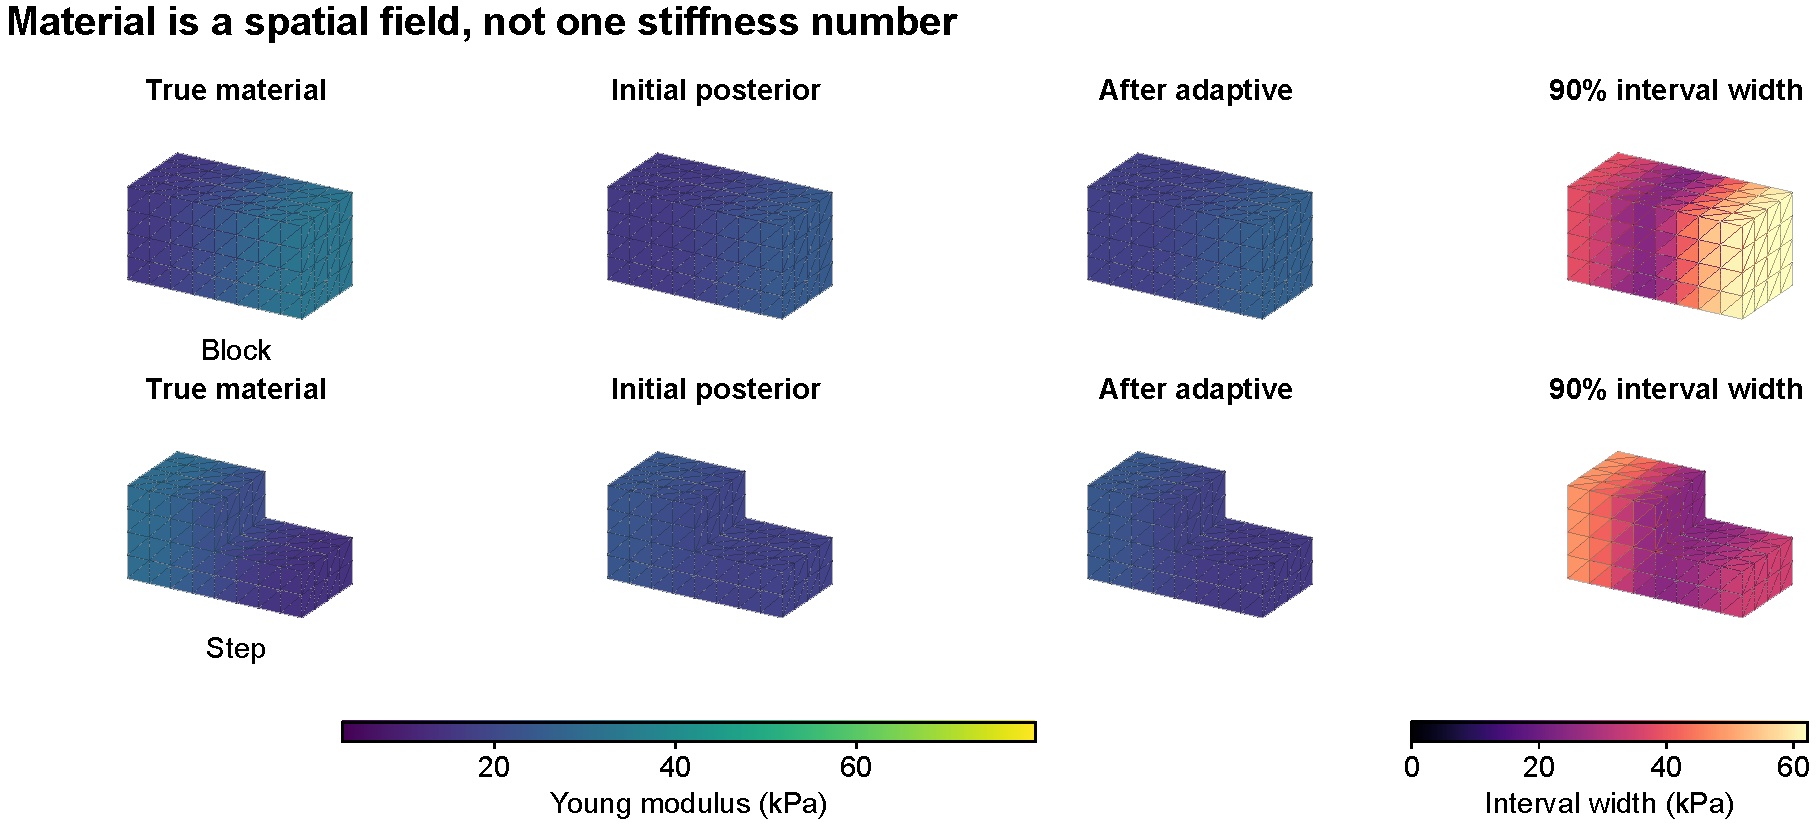
\includegraphics[width=.98\textwidth]{figures/material-fields.pdf}
\caption{\textbf{Material estimates and remaining uncertainty.} Fixed case zero, shared modulus scale and true geometry. These inferred fields can remain uncertain or incorrect despite improving some response predictions. Interval widths are posterior marginal quantities, with cohort coverage evaluated separately.}
\end{figure*}
\begin{figure*}[!t]
\centering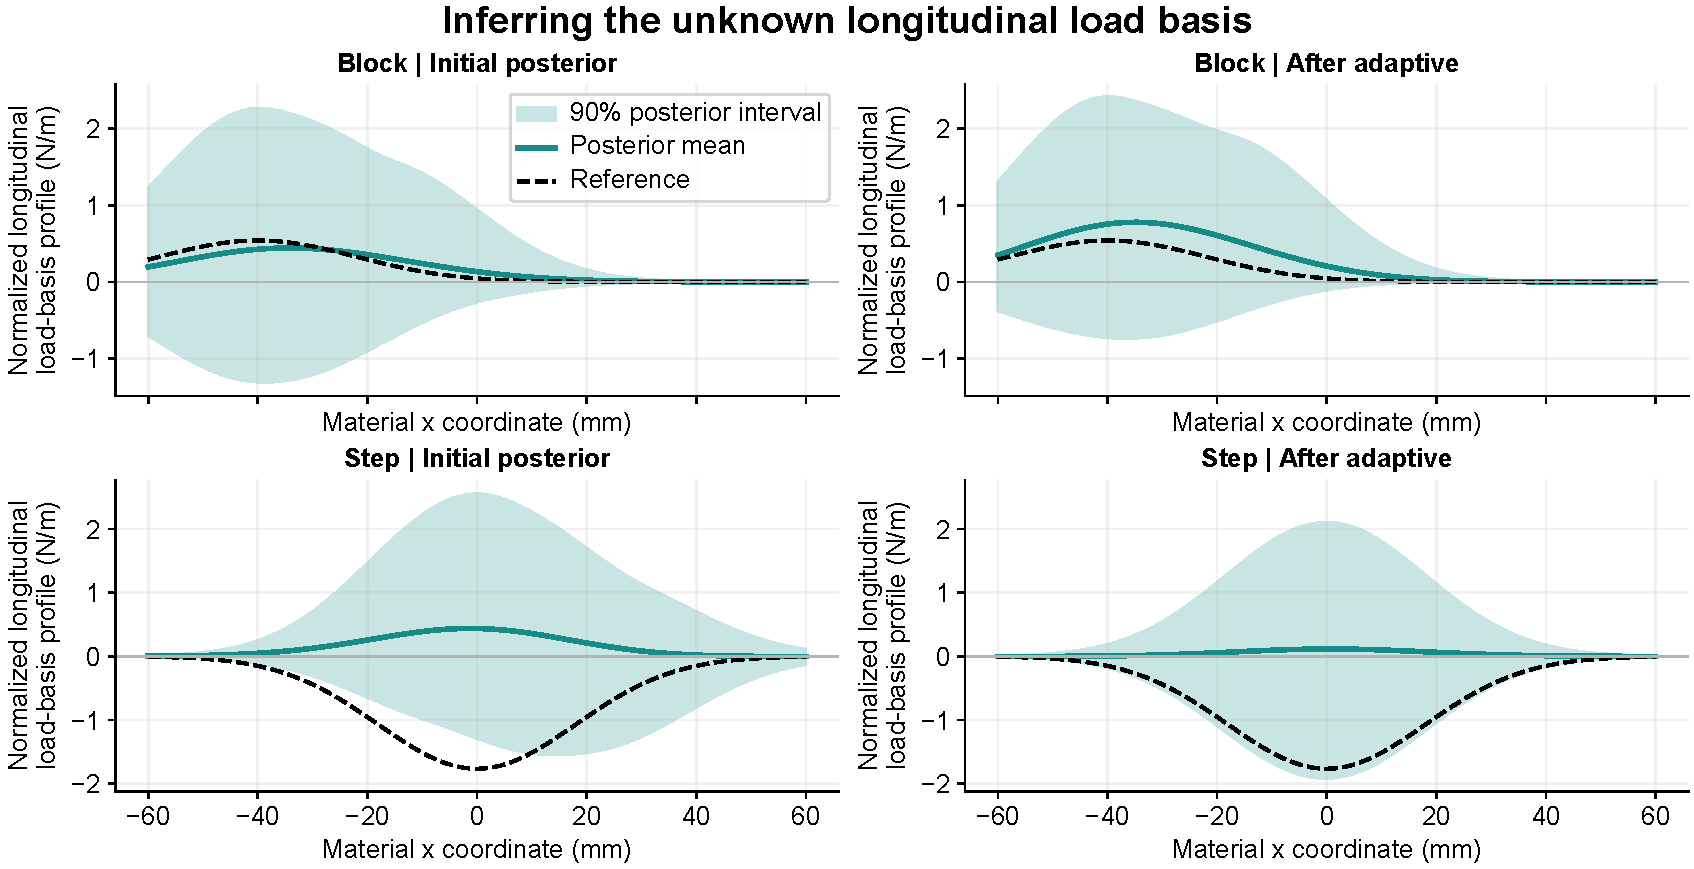
\includegraphics[width=.98\textwidth]{figures/force-fields.pdf}
\caption{\textbf{Unknown spatial loads.} Fixed case zero at the predeclared, initially unobserved time index 4. Normalized longitudinal load-basis profiles and their mixture intervals retain uncertainty in both load amplitudes and their footprint. This profile is a basis proxy: the stepped side surface has varying height, so the plotted one-dimensional normalization is not its exact surface-integrated traction. Ground truth is available only because this is a controlled synthetic experiment.}
\end{figure*}

\begin{figure*}[!t]
\centering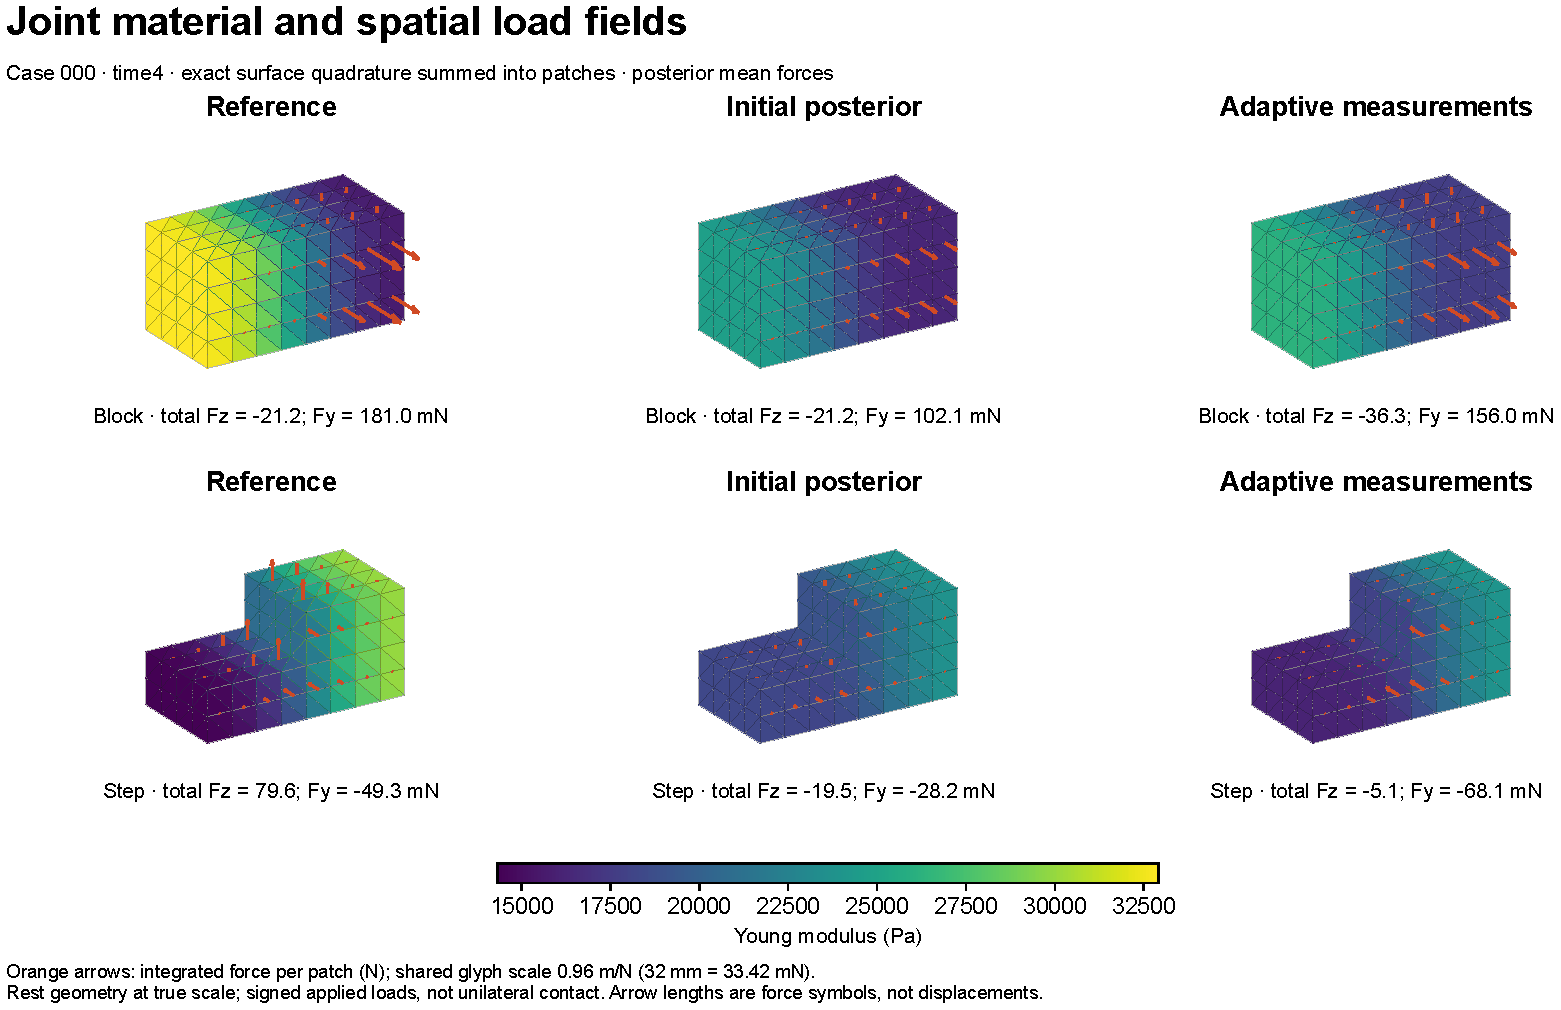
\includegraphics[width=.98\textwidth]{figures/spatial-force-fields.pdf}
\caption{\textbf{Joint material and actual surface force distributions.} Fixed case zero, time index4. Color shows inferred material modulus. Arrows show integrated force per surface patch in newtons, obtained from the exact FEM surface quadrature. All panels share an explicitly stated arrow glyph scale; this is not displacement magnification. The stepped object's posterior-mean top-force sign remains incorrect, despite improving response predictions.}
\end{figure*}

\begin{figure*}[!t]
\centering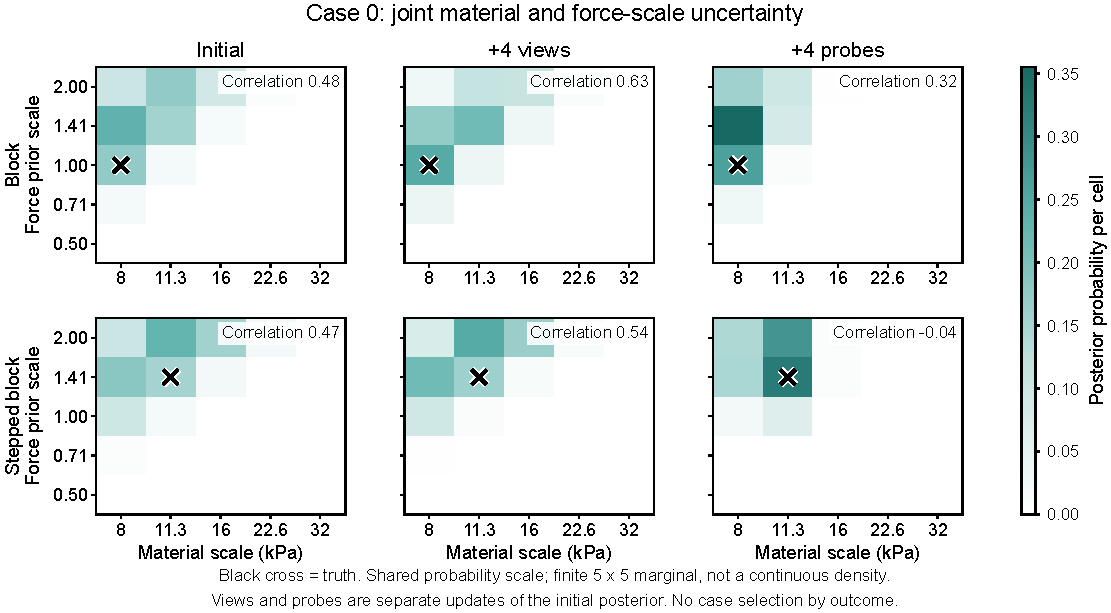
\includegraphics[width=.98\textwidth]{figures/hierarchy-joint-posterior.pdf}
\caption{\textbf{Material--force-scale dependence.} Fixed case zero in each geometry, with no outcome-based selection. The black cross marks true scale parameters. The finite 5$\times$5 marginal retains coupled explanations; cameras and probes update different aspects. Lower correlation alone is not a guarantee of more accurate identification.}
\end{figure*}
\begin{figure*}[!t]
\centering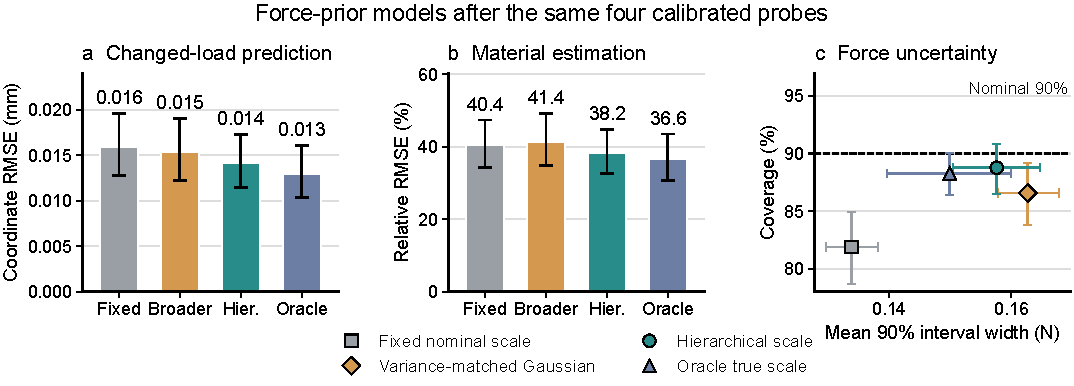
\includegraphics[width=.98\textwidth]{figures/hierarchy-prior-models.pdf}
\caption{\textbf{Force-prior controls on all 128 fresh cases.} The broader Gaussian matches the hierarchy's prior variance. Oracle receives the true amplitude scale. Error, interval coverage and width must be read together; a broader interval alone is not a successful recovery.}
\end{figure*}


\section{Excitation and forward-model qualification}
A development study compared weak, intermediate and strong Gaussian supports before freezing the final cohort. Weak supports produced mostly rigid motion. The chosen 4--16 kN/m range raises median nonrigid/total RMS to 19.5\% for block and 28.2\% for step at the tested corner loads. Representative simultaneous 0.08 N loads give maximum principal strains 2.02\%/2.61\% and maximum rigid rotations 0.0173/0.0237 rad. These deterministic cases are not bounds on an untruncated Gaussian distribution.

A post-generation audit retains all 320 original surface-study truth histories. Maximum absolute principal strain is 4.30\%, median case maximum 0.77\%, and 95th percentile 1.90\%; no case exceeds 5\%. The smallest deformation-gradient determinant is 0.982. In the independent force-scale cohort, maximum strain is 8.18\%, three of 128 cases exceed 5\%, and none exceeds 10\%; the smallest determinant is 0.958. These are checks on the declared linear generator, not validation against nonlinear elasticity.

A further development-only balanced-traction check was not promoted to replace the main action family. Opposing loads can reduce resultant force but introduce torque; three-patch loads can cancel both. At equal total absolute actuator-force budget, a greater deformation fraction often coincided with a smaller absolute signal near the observation noise. Jacobian improvements depended on geometry and measurement location. This negative diagnostic guards against assuming that visually more deformable excitation always produces better identification.

Refinement checks use medium, fine and further-refined meshes at fixed physical parameters. The last$12\to 16$cell differences range from 0.008 to 0.068 mm; primary$8\to 16$differences range from 0.027 to 0.209 mm. Hence some same-model inference errors are below discretization error. The fine-truth cohort exposes this limitation rather than treating same-mesh agreement as continuous-time or continuum physical accuracy.

\section{Finer-mesh inverse reference}
A separately frozen numerical study compares an $8\times4\times4$ inverse model with a $24\times12\times12$ model on independent $32\times16\times16$ truth. Material contrast is volume-centered consistently across meshes. Stiffness factorizations are reused across force centers, but the physical model and parameter dictionary remain unchanged. Sixteen fresh cases per geometry use the same four-action budget and fixed target. This v03 diagnostic retains interior material sensors and is not a visible-surface camera experiment. It isolates discretization effects rather than pooling its errors with the v04 surface study.
\IfFileExists{sections/fine-results.tex}{On 32 fresh high-resolution truths, initial coordinate RMSE is 0.0687\,mm for the coarse inverse model and 0.0670\,mm for the finer model. After their respective four adaptive measurements, errors are 0.0415/0.0403\,mm and nominal 90\% coverages are 76.7\%/87.2\%. Active actions may differ across inverse models; fixed schedules and potential observation noise remain paired. This comparison tests numerical model mismatch with interior sensors, not raw-video performance.
\begin{table*}[!t]\centering\small\setlength{\tabcolsep}{4pt}
\caption{Paired coarse/fine inverse reference on 32 independently generated 32-mesh truths. Both inverse models use the same 3125 parameter atoms. Sensors are interior material coordinates.}
\begin{tabular}{llrrrrr}\toprule
Inverse & Evidence & Total mm & Hidden mm & New-load mm & Material rel. & Pred. cov.\\\midrule
coarse8 & initial & 0.0687 & 0.0888 & 0.0325 & 0.457 & 78.1\\
fine24 & initial & 0.0670 & 0.0868 & 0.0306 & 0.456 & 85.2\\
coarse8 & active & 0.0415 & 0.0537 & 0.0205 & 0.378 & 76.7\\
fine24 & active & 0.0403 & 0.0521 & 0.0184 & 0.353 & 87.2\\
coarse8 & fixed & 0.0446 & 0.0581 & 0.0202 & 0.388 & 80.3\\
fine24 & fixed & 0.0417 & 0.0548 & 0.0175 & 0.361 & 88.2\\
coarse8 & fixed-view & 0.0502 & 0.0613 & 0.0297 & 0.424 & 77.2\\
fine24 & fixed-view & 0.0476 & 0.0581 & 0.0281 & 0.418 & 85.9\\
coarse8 & fixed-probe & 0.0615 & 0.0847 & 0.0169 & 0.390 & 71.9\\
fine24 & fixed-probe & 0.0599 & 0.0831 & 0.0120 & 0.299 & 86.6\\
coarse8 & random & 0.0534 & 0.0704 & 0.0206 & 0.390 & 75.8\\
fine24 & random & 0.0510 & 0.0681 & 0.0168 & 0.355 & 85.9\\
\bottomrule\end{tabular}
\end{table*}}{}

\section{Implementation, provenance and reproduction}
All priors, dictionary bounds, source hashes, case counts, observation/action/target contracts and seeds were frozen before final cohort execution. Source changes invalidate resume. Case-level records retain every policy and every acquisition score. Continuous runs retain stage histories, invalid-state counts and independent seed/count comparisons. Raw trajectory dictionaries and posterior checkpoints remain local; compact tables, source, provenance and figures are publishable without raw recordings.

The core unit suite checks rigid-mode strain, stiffness symmetry/positivity, force quadrature, gradients, CPU/GPU parity, affine interpolation, Gaussian marginal/conditional identities, covariance propagation, observation-order invariance, predictive-risk integration and strict target separation. The independent audit verifies that planners do not receive true parameters or unacquired measurements. Tests establish implementation identities and declared data flow, not real-world physical truth.

The force-elimination predecessor used a nonlinear Neo-Hookean trajectory and sparse rendered RGB. Its fifteen force coefficients were integrated exactly under a fixed full-rank velocity discrepancy model; a local Gaussian approximated the remaining trajectory/material posterior. It had no unknown spatial load footprint. Exact elimination therefore coexisted with approximate uncertainty and nonlinear renderer failures. The present reference deliberately separates these issues.

\paragraph{Historical evidence identifiers.}
The platform summary is traceable to \texttt{papers/cvpr2027-physical-response/main.tex}, its unchanged appended supplement, and \texttt{evidence/current-audit.json}. The six-family simulation table reports 1.97/10.80/11.27/1.84 mm for the neural continuum, adapted PhysTwin, adapted Spring-Gaus and analytic continuum controls. The real continuation and transfer tables are generated from \texttt{evidence/external-numbers.json} and the saved per-sequence tables. These are archived system-specific results, not new joint-field comparisons. The source package preserves those documents through the archived PDF; the repository retains all original reports.

\section{Scope of the preserved studies}
The following archived supplement is reproduced unchanged so that earlier contact, boundary, rendering and public-data evidence remains available. Its numbering, captions and methodological distinctions belong to that earlier manuscript. In particular, its learned material decoder, equilibrium real-data adapter, slip-aware SoftVT predictor, dense PIDG hybrid and solver-driven appearance qualification are distinct systems. They are not interchangeable baselines for the new finite/continuous posterior and do not establish its material/force recovery on real video.

\paragraph{Archived platform evidence.}
The unchanged historical supplement follows the new study. Its figures, numbering and comparisons belong to the earlier platform manuscript. References for the new identification study are listed in the main manuscript.
\end{document}
